% !TEX TS-program = LuaLaTeX-shell

\documentclass[convert,tikz,border=5pt]{standalone}
\usepackage{tikz}
\usetikzlibrary{positioning,shapes.multipart}
\tikzset{my node/.style={draw,thick,font=\sffamily\strut, align=center,text width=3cm,minimum height=2cm,rounded corners,fill=#1}}
\begin{document}
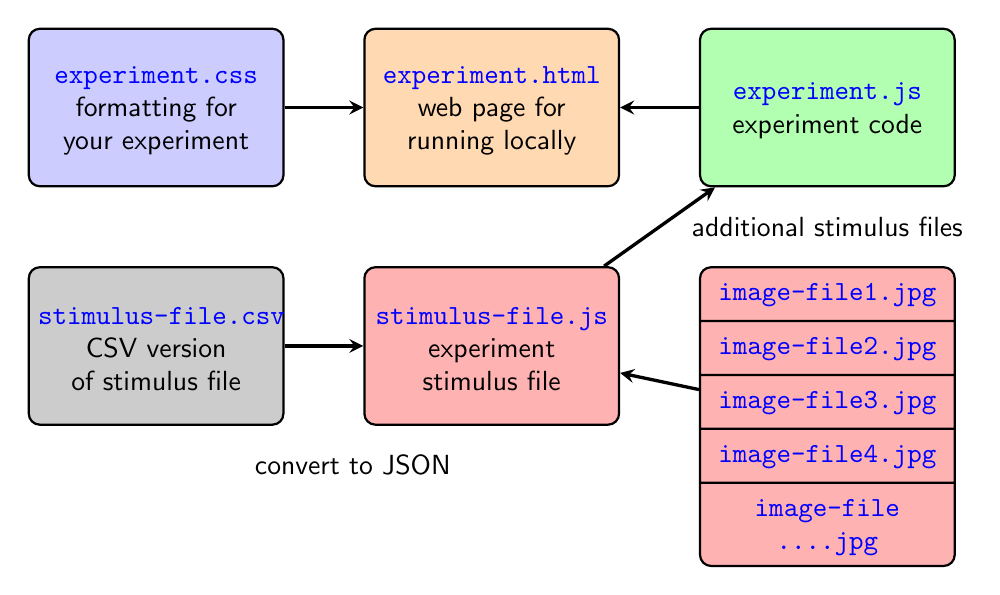
\begin{tikzpicture}
\node[my node=orange!30] (A) {{\color{blue}\texttt{experiment.html}}\\web page for running locally};
\node[my node=blue!20] (B) [left=1cm of A] {{\color{blue}\texttt{experiment.css}}\\formatting for your experiment};
\node[my node=green!30] (C) [right=1cm of A] {{\color{blue}\texttt{experiment.js}}\\experiment code};
\node[my node=red!30] (D) [below=1cm of A] {{\color{blue}\texttt{stimulus-file.js}}\\experiment stimulus file};
\node[my node=black!20] (F) [left=1cm of D] {{\color{blue}\texttt{stimulus-file.csv}}\\CSV version of stimulus file};
\node[my node=red!30,shape=rectangle split, rectangle split parts = 5] (E) [below=1cm of C] {
\nodepart{one}{\color{blue}\texttt{image-file1.jpg}}
\nodepart{two}{\color{blue}\texttt{image-file2.jpg}}
\nodepart{three}{\color{blue}\texttt{image-file3.jpg}}
\nodepart{four}{\color{blue}\texttt{image-file4.jpg}}
\nodepart{five}{\color{blue}\texttt{image-file \dots.jpg}}
};
\node [above= .25cm of E]{\sffamily additional stimulus files};
\node [below right =.25cm and -.5cm of F]{\sffamily convert to JSON};
\draw[very thick,-stealth] (B) -- (A);
\draw[very thick,-stealth] (C) -- (A);
\draw[very thick,-stealth] (D) -- (C);
\draw[very thick,-stealth] (E) -- (D);
\draw[very thick,-stealth] (F) -- (D);
\end{tikzpicture}
\end{document}